\documentclass[12pt]{article}
\usepackage{amssymb,amsmath,natbib,graphicx,amsthm,
  setspace,sectsty,anysize,times,dsfont,enumerate}

\usepackage[svgnames]{xcolor}

\usepackage{lscape,arydshln,relsize,rotating,multirow}
\usepackage{caption}
\captionsetup{%
  font=small,
  labelfont=normalfont,
  singlelinecheck=false,
  justification=justified
}
\usepackage{algorithm,algorithmic}

\newtheorem{prop}{\sc Proposition}[section]
\newtheorem{theorem}{\sc Theorem}[section]
\newtheorem{definition}{\sc Definition}[section]
\newtheorem{lemma}{\sc Lemma}[section]
\newtheorem{corollary}{\sc Corollary}[section]

\marginsize{1.1in}{.9in}{.3in}{1.4in}

\newcommand{\nb}{\color{blue}}
\newcommand{\dbl}{\setstretch{1.5}}
\newcommand{\sgl}{\setstretch{1.4}}

\newcommand{\bs}[1]{\boldsymbol{#1}}
\newcommand{\mc}[1]{\mathcal{#1}}
\newcommand{\mr}[1]{\mathrm{#1}}
\newcommand{\bm}[1]{\mathbf{#1}}
\newcommand{\ds}[1]{\mathds{#1}}
\newcommand{\indep}{\perp\!\!\!\perp}
\DeclareMathOperator*{\argmin}{argmin}
\newcommand{\norm}[1]{|\!|#1|\!|_{1}}
\newcommand{\code}[1]{{\smaller\sf#1}}
\newcommand{\e}[1]{{\footnotesize$\times10$}{$^{#1}$}}

\usepackage[bottom,hang,flushmargin]{footmisc}

\pdfminorversion=4
\begin{document}

\sgl 

\pagestyle{empty}

\noindent {\Large \bf Comment: \textit{Coauthorship and citation networks for
statisticians}} 

\vskip .5cm

\noindent{\large Mladen Kolar -- University of Chicago Booth School of Business\\Matt Taddy -- 
{Microsoft Research and Chicago Booth}}

 

\vskip 1cm\noindent This article by Ji and Jin (JJ throughout)
provides a network analysis, by two experts in the field, on the
connections between statisticians and statistics research papers.
This is not just an exercise in navel-gazing, but also an opportunity
to compare results obtained by different methods in an area we know
well: our profession.  We think that the article leads to  lessons
for how we use network models and what data we choose to analyze.
First, one can gain insight into a network by considering meta-information
for the nodes -- in this case, the research paper abstracts. Second, 
since summary statistics like closeness and betweenness centrality are sensitive to partial network observation, one needs to take care in defining the universe of nodes.  

\subsection*{Topic analysis}


In our first study, we consider decomposing the abstracts of the articles into latent `topics', e.g., as in the LDA of \cite{blei_latent_2003}.  The properties of the citation network can then be considered in light of the topical {\it content} of the articles.
We use the {\tt maptpx} R package \citep{taddy_estimation_2012} to obtain posterior maximizing point estimates for LDA topics.  The {\tt maptpx} package applies the Bayes factors of \cite{taddy_estimation_2012} in model selection, and for this data we find that a 15 topic decomposition is optimal. The full code to fit this model (and all of our other analyses) and to generate summaries is at {\tt https://github.com/TaddyLab/statsArticles}.  


\begin{figure}
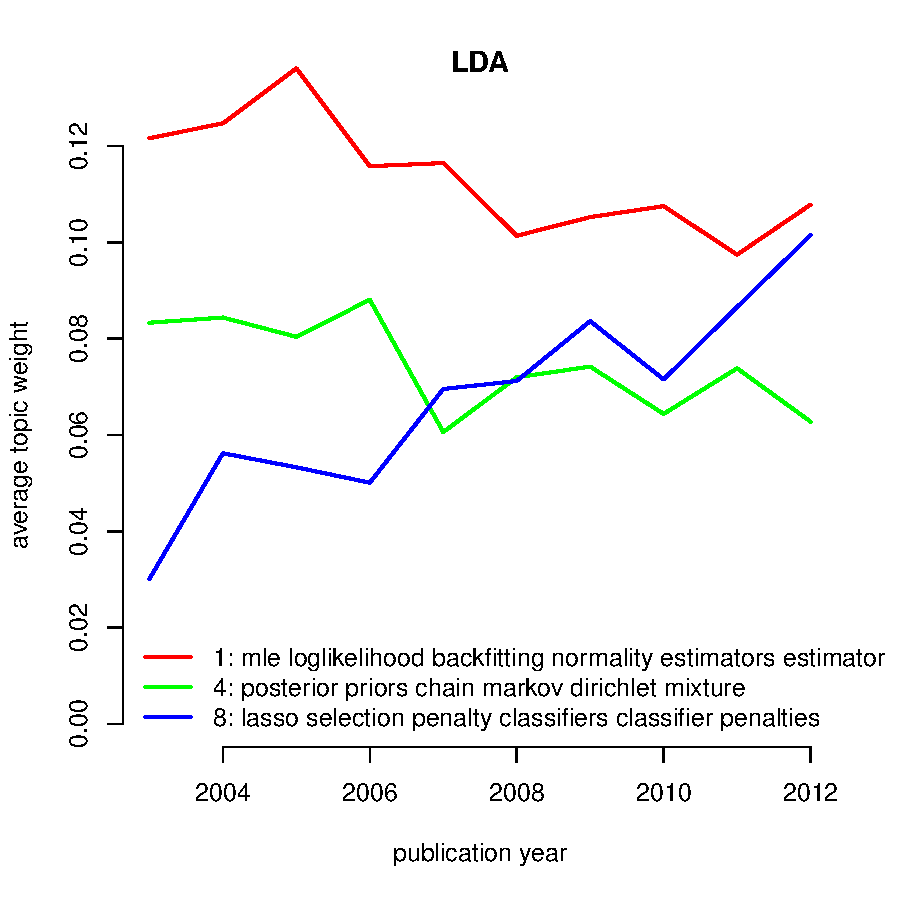
\includegraphics[width=0.5\textwidth]{lda}
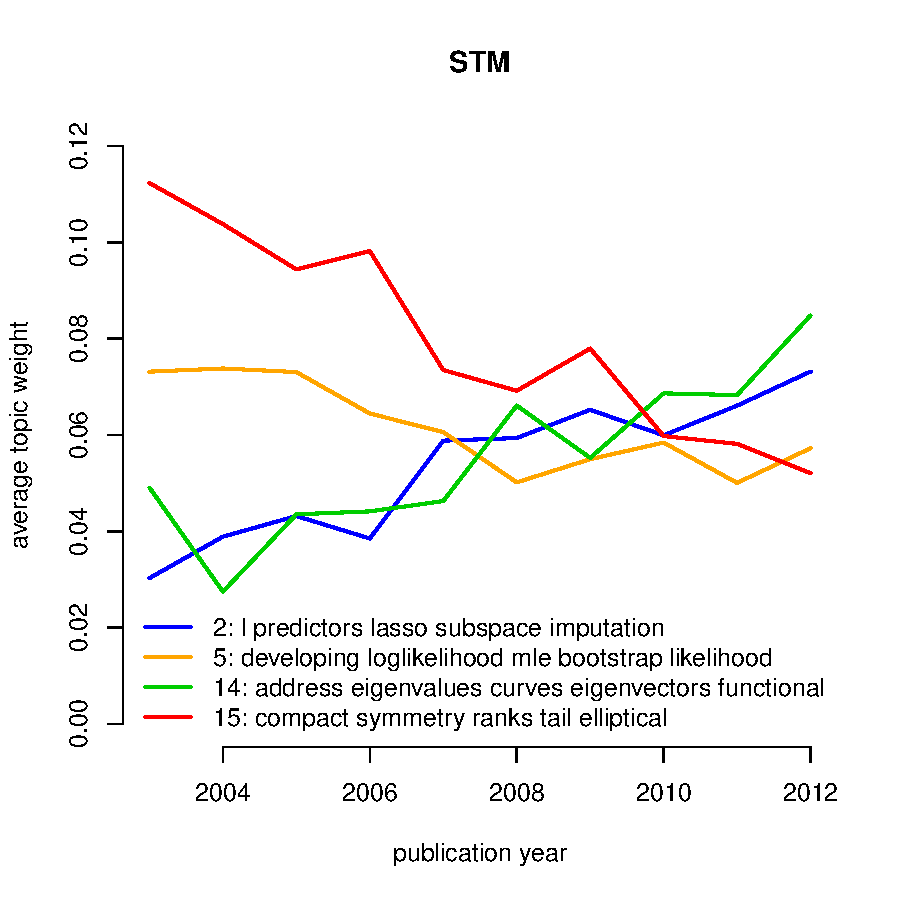
\includegraphics[width=0.5\textwidth]{stm}
\caption{\label{fig:topics} Annual average document-topic weights (that proportion of document devoted to each topic) for topics that saw their usage change by more than 0.1 between the first and last five years of our sample.  The left panel shows  topics from LDA via {\tt maptpx} and the right shows topics from STM via {\tt stm}. }
\end{figure}

We focus on topics that have seen their usage change over time -- their
mean proportions within documents during the first and last five years
differ by more than 0.01.  Most topics were stable over time, so that
only three meet this threshold.   These three topics are shown in
the left panel of Figure \ref{fig:topics}.  The list of words given for each topic are those with the highest {\it lift}: within-topic probability over the average corpus-wide occurrence rate.  

Topic 1 seems to contain traditional mathematical statistics content, especially for non and semi parametric analysis.  The three articles most representative of this topic (i.e., have the highest estimated usage) are 

{\it Backfitting and smooth backfitting for additive quantile models} \citep{lee2010backfitting}

{\it Depth weighted scatter estimators} \citep{zuo2005depth}, and

{\it Estimating invariant laws of linear processes by U-statistics} \citep{schick2004estimating}.

\noindent
This topic remains relatively popular, but its usage is decreasing over time.
The other topic that is decreasing in popularity, topic 4, appears to represent Bayesian analysis.  Its three most representative articles are

{\it A conjugate prior for discrete hierarchical log-linear models} \citep{massam2009conjugate}

{\it Bayesian analysis of variable-order, reversible {M}arkov chains}
\citep{bacallado2011bayesian}

{\it Recapture models under equality constraints for the conditional capture probabilities
} 

\vskip -.25cm
\citep{farcomeni2011recapture}

\noindent
 Over the same time period, we see a dramatic rise in the prevalence of topic 8, which appears to represent the material related to the popular penalized-deviance 
estimation framework. Its three most representative articles are

{\it The adaptive lasso and its oracle properties} \citep{Zou2006adaptive}

{\it Regularization and variable selection via the elastic net} \citep{zou2005regularization}

{\it On the adaptive elastic-net with a diverging number of parameters} \citep{Zou2009adaptive}

\noindent
Thus, our topic model shows an increased interest in penalized deviance estimation (and techniques popular in both statistics and machine learning).  This rise in popularity for topic 8 has come at the expense of  Bayesian analysis and another topic that is roughly interpretable as a different flavor of flexible analysis.  Certainly, our personal experience supports the loss of market share for fully Bayesian analysis; as datasets have grown in size we are often maximizing posteriors (which yields penalized deviance estimators) rather than averaging over them \citep[][are personal examples]{taddy_estimation_2012,taddy_one-step_2015}.

This topic decomposition can be related back to the document networks.  For example, we might be interested in which topics tend to generate higher citations.  A linear regression of citations per year (the total count divided by the years since publication) onto a year indicator (i.e, a publication-date-specific intercept) and the document-topic weights yields an estimated extra 0.1 citations for  per extra 0.1 weight  on topic 8, our penalized deviance topic. This has a $z$-value of around 100, and it is the {\it only} topic that has a significant effect on citations.   Note that this is only the 8th most common topic in our sample, so that the higher cite count is not explainable by prevalence.  It is impossible to tell whether the topic is gaining popularity because it tends to lead to citations, or (what seems more likely) if these papers are cited often because the topic is becoming popular.

Our analysis above follows a simple two-stage procedure: we first estimate the topics and then relate them to network statistics (cite counts, i.e., degree in the citation network).
A more complex procedure, such as the recent work by \cite{TanChanZheng2015}, could be used to jointly estimate network communities and text topics (e.g., to see if authors tend to cite within rather than across topics).  As a partial step in this direction, we also applied the structural topic model (STM) of \cite{roberts2013structural} as implemented in the {\tt stm} package for R \citep{roberts2014stm}.  STM assumes that document-topic proportions are generated around a linear function of document attributes.  Applying STM with both citations-per-year and publication date (annual indicators) as inputs yields the topics in the right panel of Figure \ref{fig:topics}.  We  used 15 topics, as in our earlier LDA.  Again, a topic that focuses on penalized deviance estimation shows the biggest gains in usage over time.  Two other topics are also gaining in popularity: one focused on classification (perhaps including much of the machine learning material that was also included in LDA's topic 8) and another that is tough for us to interpret.  There is only one big loser over time: topic 15, which is also tough to interpret.  

Across both models, STM and LDA, the point of clear agreement is that penalized deviance estimation is a well-defined topic that is gaining in popularity.  As we found in our two stage estimation, this topic is associated with higher citations: the fitted STM has a posterior mean effect of an extra 0.5 citations-per-year for an extra 0.1 usage of the penalized deviance topic.

\subsection*{Sensitivity of the citation networks to journal choice}

One issue for JJ's analysis is that it includes only a small
portion of the statistics publication venues.  Excluded are any applied
journals (except for the Applications and Case Studies section of JASA),
journals from other fields that use statistics and cite statistical research,
and the entire machine learning literature.  Certain network statistics, such
as the betweenness centrality scores, are especially sensitive to any
missingness in the network.  However, as already pointed out by JJ, even simple
 degree statistics (i.e., citation counts) are sensitive to the set of
journals considered. We illustrate how the set of journals in the dataset affects
the hot papers by removing all Biometrika or all JRSS-B papers. There are
total of 751 papers published in Biometrika and 411 in JRSS-B during the
period considered.



%%%%%%%%%%%%%%
%%%%%%%%%%%%%%
%%%%%%%%%%%%%%
\begin{table}[htb]
\centering
\caption{``Hot" papers (alphabetically) identified  by degree centrality (Column 2; for citation networks of papers), closeness centrality, and betweenness centrality, when papers
  published in Biometrika are removed.   Numbers in column $2$-$4$ are the ranks (shown when the rank is   smaller than or equal to $5$).}
\scalebox{0.875}{
\begin{tabular}{l|ccc}
Paper                                                &  Citations  & Closeness & Betweenness \\
\hline
\cite{Bunea2007Aggregation}   &    &    & 4 \\
\cite{Candes2007Dantzig}      &  3 &    & \\
\cite{Fan2004New}             &    &  3 & \\
\cite{Fan2008Sure}            &    &    & 1 \\
\cite{Fan2004Nonconcave}      &  4 &  1 & \\
\cite{Genovese2004stochastic} &  5 &    & \\
\cite{Huang2008Asymptotic}    &    &    & 2 \\
\cite{Johnstone2004Needles}   &    &  4 & \\
\cite{Koltchinskii2006Local}  &    &    & 5 \\
\cite{Meinshausen2006High}    &  2 &  5 & \\ 
\cite{Storey2004Strong}       &    &  2 & \\
\cite{Zou2006adaptive}        &  1 &    & \\
\cite{Zou2008One}             &    &    & 3 \\
\hline
\end{tabular}
\label{tab:hotPapers}
}
\end{table}
%%%%%%%%%%
%%%%%%%%%%
%%%%%%%%%%
%%%%%%%%%%


% \begin{table}[htb!]
% \centering
% \caption{Top $3$ authors identified by the degree centrality (Columns $1$-$3$; corresponding networks are  the author-paper bipartite network, Coauthorship  network, and Citation network for authors),    the closeness centrality and the betweenness centrality. JRSSB removed.}
% \scalebox{0.92}{
% \begin{tabular}{|lllll|}
% \hline
% $\#$ of papers    &  $\#$ of coauthors & $\#$ of citers     & Closeness            & Betweenness \\
% \hline
% Peter Hall  &  Peter Hall  &  Jianqing Fan  &  Raymond Carroll  &  Raymond Carroll   \\ 
% Jianqing Fan  &  Raymond Carroll  &  Hui Zou  &  Peter Hall  &  Peter Hall  \\ 
% Raymond Carroll  &  Joseph Ibrahim  &  Nicolai Meinshausen  &  Jianqing Fan  &  Runze Li  \\ 
% \hline
% \end{tabular}}
% \label{tab:keyAuthors:jrssb}
% \end{table}



%%%%%%%%%%%%%%
%%%%%%%%%%%%%%
%%%%%%%%%%%%%%
\begin{table}[htb!]
\centering
\caption{``Hot" papers (alphabetically) identified  by degree centrality (Column 2; for citation networks of papers), closeness centrality, and betweenness centrality, when
  papers published in JRSS-B are removed.   Numbers in Column $2$-$4$ are the ranks (only shown when the rank is   smaller than or equal to $5$).}
\scalebox{0.875}{
\begin{tabular}{l|ccc}
Paper (Area)                                                &  Citations  & Closeness & Betweenness \\
\hline
\cite{Bickel2008Covariance}   &    &    & 4 \\
\cite{Bunea2007Aggregation}   &    &    & 3 \\
\cite{Candes2007Dantzig}      &  3 &    & \\
\cite{Drton2004Multimodality} &    &  4 & \\
\cite{Drton2004Model}         &    &  5 & \\
\cite{Fan2004Nonconcave}      &  4 &  1 & \\
\cite{Genovese2004stochastic} &  5 &    & \\
\cite{Huang2006Covariance}    &    &    & 2 \\
\cite{Hunter2005Variable}     &    &  2 & \\
\cite{Johnstone2004Needles}   &    &  3 & \\
\cite{Koltchinskii2006Local}  &    &    & 5 \\
\cite{Meinshausen2006High}    &  2 &    & \\ 
\cite{Zou2006adaptive}        &  1 &    & \\
\cite{Zou2008One}             &    &    & 1 \\
\hline
\end{tabular}
\label{tab:hotPapers:jrrsb}
}
\end{table}
%%%%%%%%%%
%%%%%%%%%%
%%%%%%%%%%
%%%%%%%%%%

Table~\ref{tab:hotPapers} presents ``hot'' papers when publications from Biometrika are removed from the network.  The top 5 hot articles as measured by the number of citations (i.e., by degree) stays
almost the same as in Table 3 of JJ. \cite{zou2005regularization} at
5th place is replaced by \cite{Genovese2004stochastic} (which is
ranked 6th when considering all 4 journals). When using
closeness centrality, \cite{Meinshausen2006High} ranks 5th (originally
it was ranked 9th), while \cite{Hunter2005Variable} falls to 6th
place.  Finally, when using betweenness centrality
\cite{Bunea2007Aggregation} and \cite{Koltchinskii2006Local} are ranked 
in the top 5, while initially they were not ranked in the top 10 papers.

Table~\ref{tab:hotPapers:jrrsb} shows the inferred ``hot'' papers when publications from JRSS-B are removed from the network. Ranking based on citation count gives
us the same ordering as when papers published in Biometrika were
removed.  However, when looking at ranking based on closeness
centrality, we observe that \cite{Drton2004Multimodality} and
\cite{Drton2004Model} are ranked 4th and 5th, while before they were
not in the top 5. Again, using betweenness centrality
\cite{Bunea2007Aggregation} and \cite{Koltchinskii2006Local} are
ranked in the top 5.

We see here that both betweenness and degree rankings, even at the very top ranks, are sensitive  to changes in journal set.  This type of behavior is well known
\citep[e.g.,][]{Borgatti2006robustness}, but seeing it in practice is a good reminder: any conclusions you make about network centrality are  valid only for the {\it observed} network.   Thus, JJ's results are relevant only for the research universe defined by this small set of largely theoretical journals. We look forward to forthcoming
study by the authors, studying a larger set of journals, that might provide more general insights into our
profession.



% \begin{table}[htb!]
% \centering
% \caption{Top $3$ authors identified by the degree centrality (Columns $1$-$3$; corresponding networks are  the author-paper bipartite network, Coauthorship  network, and Citation network for authors),    the closeness centrality and the betweenness centrality. Biometrika removed.}
% \scalebox{0.92}{
% \begin{tabular}{|lllll|}
% \hline
% $\#$ of papers    &  $\#$ of coauthors & $\#$ of citers     & Closeness            & Betweenness \\
% \hline
% Peter Hall  &  Peter Hall  &  Jianqing Fan  &  Peter Hall  &  Peter Hall    \\ 
% Jianqing Fan  &  Raymond Carroll  &  Hui Zou  &  Raymond Carroll  &  Raymond Carroll   \\ 
% Tony Cai  &  Joseph Ibrahim  &  Peter Hall  &  Jianqing Fan  &  Jianqing Fan   \\ 
% \hline
% \end{tabular}}
% \label{tab:keyAuthors}
% \end{table}





\setstretch{1}\small
\bibliographystyle{chicago}
\bibliography{taddy}

\end{document}
